\subsection{Mircro-controller}
As said above, we decided to create, with an Arduino Due controller, a "real life" design of our traffic lights system.

We wired LEDs to the boards to imitate the green and red lights of the system. We also added a button for the pedestrians to imitate a real call as we would want to go through a crossroad and another push-button to generate the arrival of a bus in the system. There are also what we call information LEDs that can be lighten up if we arrive in a state that is problematic, or when one call is queuing. 
We added redundant checking in the controller that checks for example that there is not conflicting green light. In this sense, we took  properties we had modelized for the Verification project and we incorporated them into our embedded system.

\begin{figure}[H]
	\label{fig:arduino}
  	\centering
    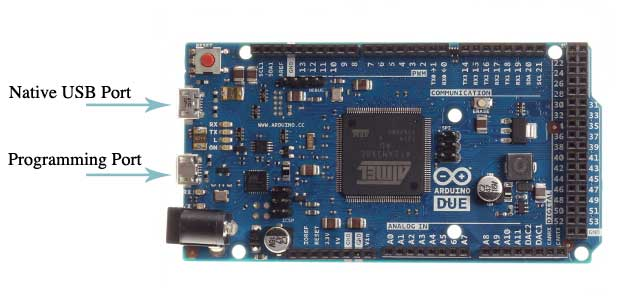
\includegraphics[width=0.4\textwidth]{picture/arduino.jpg}
    \caption{Arduino Due used for the embedded system}
\end{figure} 

To do so, we wrote the code needed for the good functioning of our system in Arduino C.